\chapter{Platform}
\head{This chapter describes the platform to introduce a system overview. This helps to understand the physical interconnections that exists between modules.}

\noindent Ths total system consists of a wide range og modules, which are different components og sensors and actuators. Theese modules are connected to a \ac{LLI} and \ac{HLI} computing device. The \ac{LLI} is a micontroller, which takes care of the basic functions of the platform, such as communicationg with basic sensors and actuators. The software for this is embedded and writen in C for avr-gcc compiler.

The \ac{HLI} is a x86 comnpatible computer of some sort that is able to run the higher abstraction layer code written in Python. This higher abstracion layer contains the onboard generation og waypoints of map data, to calculate the desired heading and speed for the vessel. This also calculates the stuff for the state space model which in turn talks to the \ac{LLI}.

Some modules that is connected to the \ac{LLI} is not handled by the \ac{LLI} itself, but forwards the data to the \ac{HLI} which uses this data for the control. A illustration of this can be seen on figure~\vref{fig:vessel-block-overview}.


\begin{figure}[htbp]
	\centering
	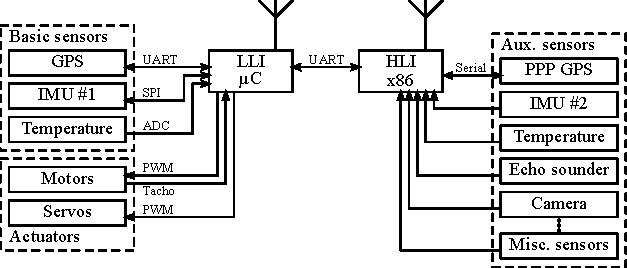
\includegraphics[width=\textwidth]{img/vessel-block-overview-electrical}
	\caption{Overview of electrical interconnections between \ac{LLI} and \ac{HLI} together with periphal modules.}
	\label{fig:vessel-block-overview-electrical}
\end{figure}
